\documentclass[../rapport_MVEX01-11-05]{subfiles}
\begin{document}

\subsection{\knn}

\begin{table}
	  \centering
		\label{tab:tolkningsmatris}
		\caption{}
    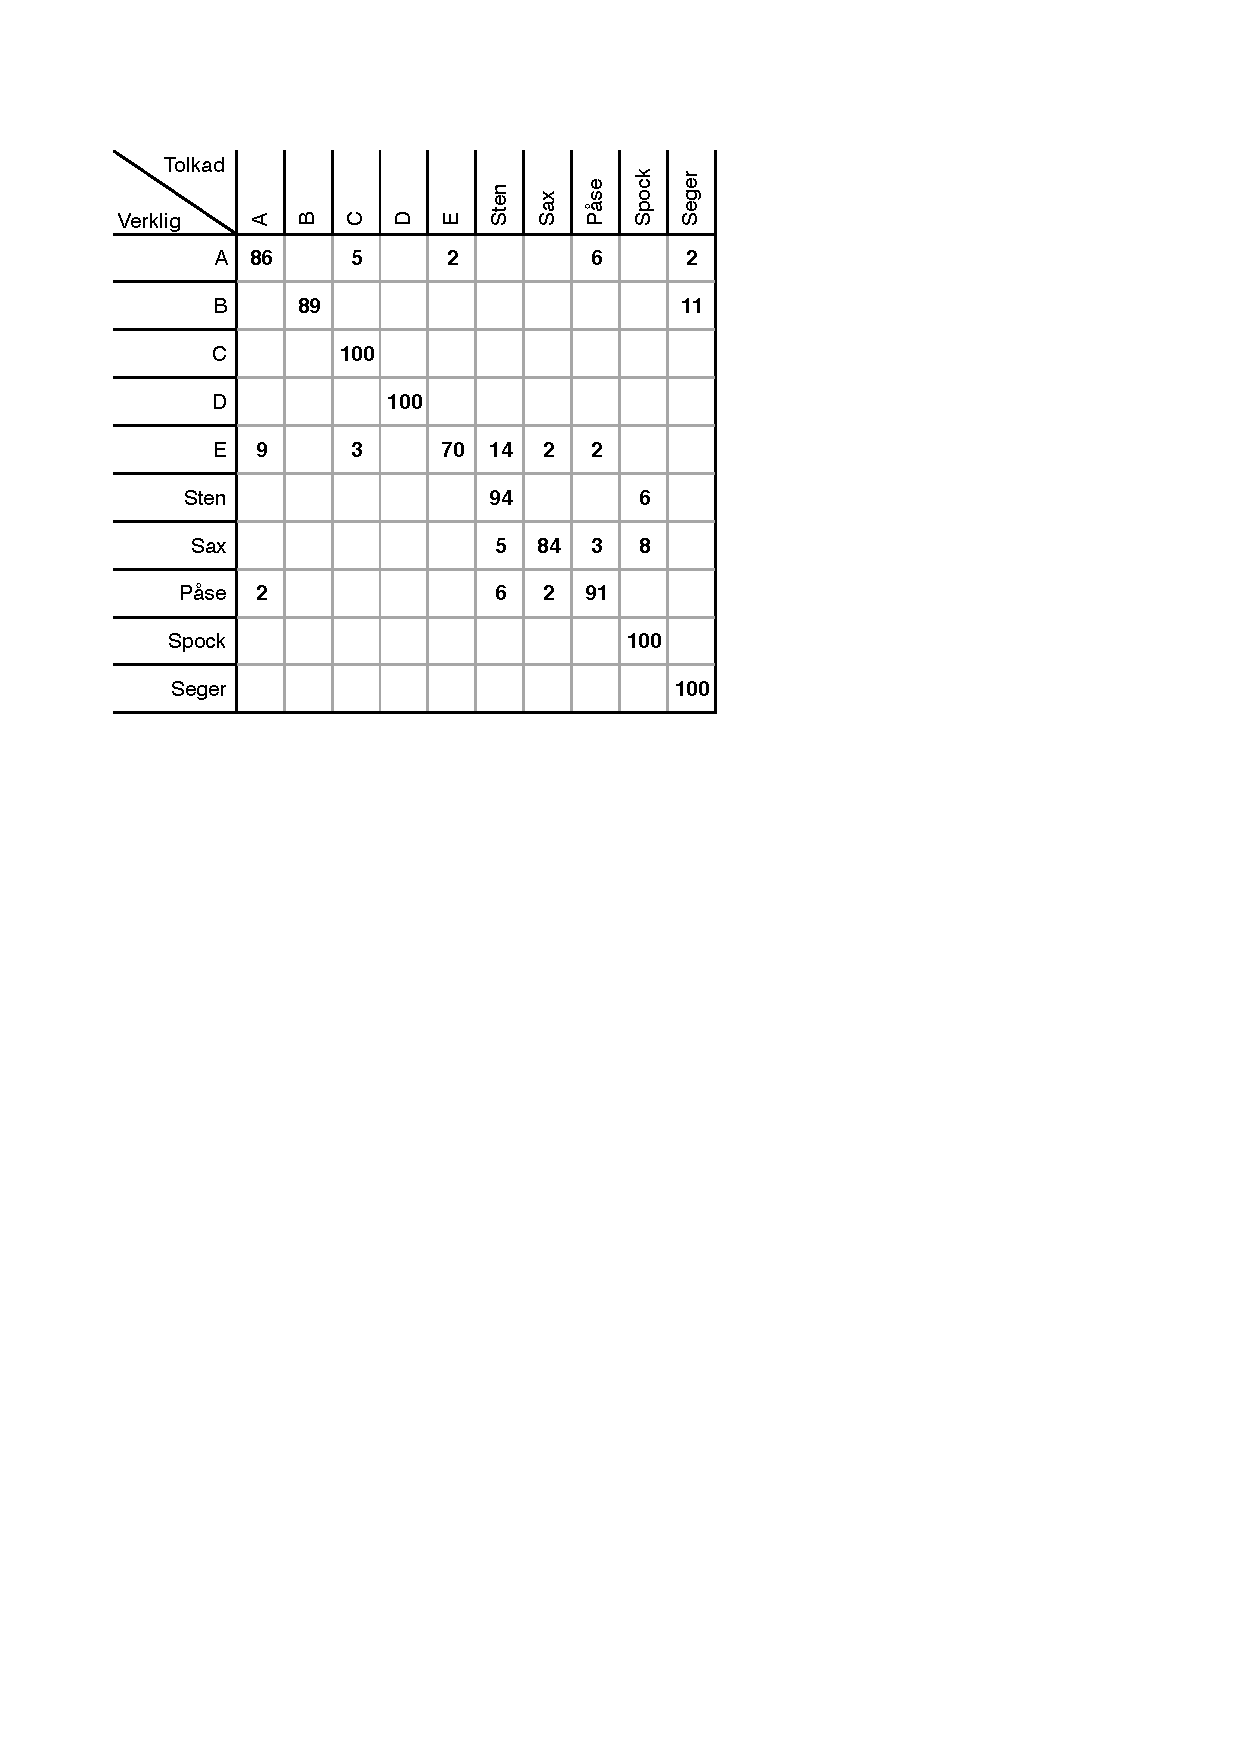
\includegraphics[trim=2cm 9cm 2cm 2.5cm]{bilder/tolkningsmatris.pdf}
		%\begin{tabular}{l|cccccccccc}
		%\backslashbox{Verklig}{Tolkad} & a & b & c & d & e & Sten & Sax & Påse & Spock & Seger\\
		%\toprule
		%a & 86 &  & 5 &  & 2 &  &  & 6 &  & 2 \\ 
		%b &  & 89 &  &  &  &  &  &  &  & 11 \\ 
		%c & &  & 100 &  &  &  &  &  &  &  \\ 
		%d &  &  &  & 100 &  &  &  &  &  &  \\ 
		%e & 9 &  & 3 &  & 70 & 14 & 2 & 2 &  &  \\ 
		%Sten & &  &  &  &  & 94 &  &  & 6 &  \\ 
		%Sax & &  &  &  &  & 5 & 84 & 3 & 8 &  \\ 
		%Påse & 2 &  &  &  &  & 6 & 2 & 91 &  &  \\ 
		%Spock &  &  &  &  &  &  &  &  & 100 &  \\ 
		%Seger & &  &  &  &  &  &  &  &  & 100 \\  
		%\end{tabular}
\end{table}

%\notes{Jag vill ha den som \LaTeX{} men inte som en ''ful'' tabell. Det verkar
%finnas ett paket \texttt{slashbox} som gör den sneda biten, i komination med
%typ \texttt{colortbl} kan det bli hyfsat okej. Men riktiga tabeller ska vi nog
%använda \texttt{booktabs till}.}

\end{document}